% !TEX encoding = UTF-8 Unicode
\chapter{La \mt Convergence Cross Mapping}
\label{chap6}

\section{M\'ethodologie}
Convergence Cross-Mapping (CCM) est une nouvelle approche méthodologique qui peut aider à détecter la causalité de la corrélation parasite dans les séries chronologiques du système dynamique \cite{sugihara2012,tsonis2015,deyle2016}. L'idée est que si une variable $\textit{Y}$ peut prédire l'état actuel ou précédent de la variable $\textit{X}$, alors $\textit{X}$ influence causalement $\textit{Y}$. Plus précisément, CCM construit d'abord deux variétés à partir de coordonnées décalées de la variable des séries temporelles $\textit{X}$ et $\textit{Y}$. Puis CCM trouve pour les signatures de $ \ textit {X} $ dans la série temporelle $\textit{Y}$ en cherchant s'il y a une correspondance entre les points de deux variétés $\textit{M}_X$ et $\textit {M}_Y$. Si l'indice temporel du point voisin sur la variété $\textit{Y}$ peut être utilisé pour identifier un point proche sur $\textit{M} _X$, alors nous pouvons utiliser $\textit{Y}$ pour estimer $\textit{X}$ et vice versa. Notez que CCM est lié à la notion générale de prédiction croisée mais avec quelques différences importantes. CCM estime d'abord les "états" des variables et ne prévoit pas comment le système "évolue" sur le variété. Après cela, le CCM implique des convergences - l'estimation croisée améliore la compétence d'estimation avec une longueur de série chronologique $\textit {L}$. La corrélation croisée est quantifiée en calculant le coefficient de corrélation $\rho$ entre les séries temporelles prédites et observées. Si la compétence de cartographie croisée augmente avec la longueur des séries chronologiques, un effet causal direct ou indirect peut être déduit. Cependant, dans certaines applications pratiques, où les variétés d'ombre sont une approximation à basse dimension du système réel, la convergence sera limitée par l'erreur d'observation, le bruit du processus et la longueur des séries temporelles $\textit{L}$.

\section{\Rs}

\subsection{\Rs d'analyse univariable}

Nous avons utilisée la méthode CCM pour tester la causalité entre la dengue et les facteurs environnementaux. Nous comparons la prédiction croisée mesurée pour chaque facteur climatique d'observation avec l'expectation nulle obtenue par cartographie croisée avec des séries temporelles de substitution ayant le même cycle saisonnier que le série observée, mais avec des anomalie aléatoire. La relation est identifiée lorsque la prédiction croisée est significatif meilleure pour le facteur environnemental réel que pour les substituts nuls. 

La figure \ref{Resultccm1} montre le résultat des distributions nulles pour la prédiction croisée  $ (\rho_{ccm}) $ classées par latitude entre la dengue et certains facteurs climatiques: température moyenne, précipitations, heures d'ensoleillement, humidité relative et humidité absolue présentée sous forme de parcelles de moustaches. Les valeurs de compétences CCM mesurées sont tracées sur le cercle de couleur (rouge et vert) qui est rouge si la valeur est significativement différente de la distribution nulle $(P \leq 0,05)$ et verte sinon. 

Selon les compétences des résultats, on peut voir que le température moyenne (TA) et l'humidité absolue(AH) forcent fortement la causalité dans la plupart des provinces du centre et du sud du Vietnam. La pluviosité (RF) et l'humidité relative (RH) impact sur des provinces au sud du Vietnam et l'heures d'ensoleillement montrent leur  effect uniquement au centre du Vietnam. Nous continuons à utiliser la méthode de Fisher pour calculer la p-valeur des  facteurs climatiques: $P \leq 0,5$ pour TA, $P \leq 0,0056$ pour RH et $P\leq 0,01$ pour SH. Le résultat de leurs trois facteurs climatiques montre le forçage important dans leurs provinces à travers la latitude. Cependant, le résultat de AH et RF ne sont pas significatifs ($P \leq 0,174$ pour AH et $P \leq 0,882$ pour RF).

\begin{figure}[h]
\begin{center}
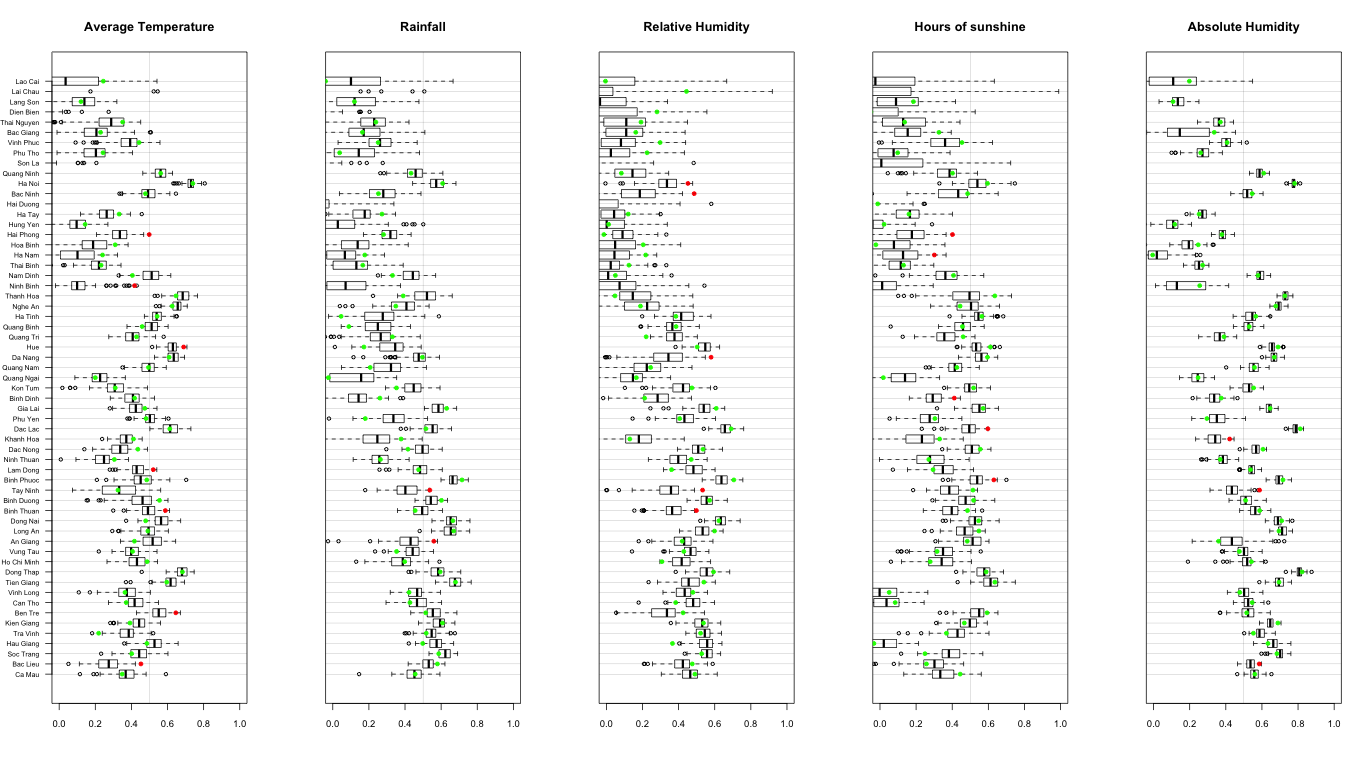
\includegraphics[width = \linewidth]{../figures/chap6/ccm_result1_100sur.png}
\caption{Detecting cross-map causality beyong shared seasonality of environmental drivers on dengue fever.}
\label{Resultccm1}	
\end{center}
\end{figure}

\subsection{\Rs d'analyse multivariable}

Pour obtenir des résultats plus détaillés, nous avons appliqué l'approche EDM multivariée pour calculer l'amélioration des prévisions en ajoutant des facteurs environnementaux supplémentaires.  Les valeurs de l'amélioration des prévisions $(\Delta\rho)$ ont été calculées par $ \Delta \rho = \rho(avec le facteur supplémentaire) - \rho(sans facteur supplémentaire)$ où $\rho$ est la corrélation de Pearson entre observations et prévisions EDM. La figure \ref{Resultccm2} montre le résultat de l’amélioration prévisionnelle de 64 provinces du Vietnam divisées par 3 régions: Nord, Centre et Sud base sur leur latitude et aussi le résultat global du Vietnam. Leurs résultats ont été classifiés par la p-valeur calculée par le test de student-t. Nous pouvons voir que la combinaison de SH et de AH montre une forte influence par rapport à leur prévision de solitude au nord du Vietnam. Ce résultat est correspond au climat subtropical humide du Nord du Vietnam. Cependant, la combinaison entre TA et AH, TA et SH montre un fort effet causal dans le climat de mousson tropical dans le centre du Vietnam. Le sud du Vietnam avec le climat tropical de la savane est moins varié que les autres régions. Avec les températures élevées tout au long de l’année, la combinaison de TA et AH, RH et AH a un impact important sur la dengue dans cette région. l’amélioration prévisionnelle de l’assistance technique et de l’assistance technique combinées a forcé la causalité sur le plan mondial au Vietnam et dans la région du centre et du sud. Dernièrement, l’amélioration prévue de TA et de AH pris ensemble a forcé la causalité au niveau mondial du Vietnam et aussi dans la région centrale et méridionale.
Ces résultats sont similés avec ceux de la méthode GCA au chapitre 5 et la méthode analyse ondelette au chapitre 4.  Ces résultats peuvent confirmer les effets énormes des facteurs météorologiques sur le développement de l'une des maladies infectieuse les plus mortelles du monde. 

\begin{figure}[h]
\begin{center}
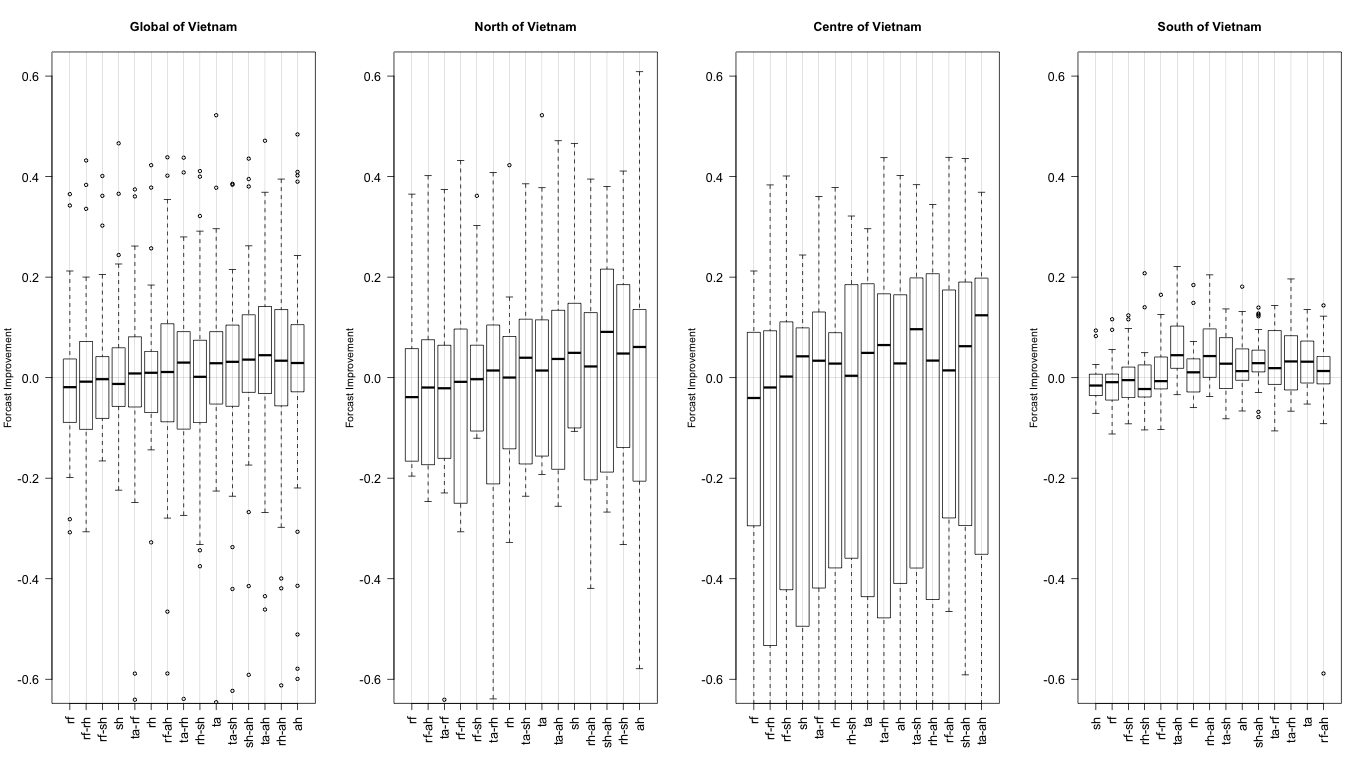
\includegraphics[width = \linewidth]{../figures/chap6/ccm_result2_n.png}
\caption{Forcast improvement with multivariate EDM. Causal effet is demonstrated if EDM forcast skill $(\rho)$ improves when a driver variables is include in the EDM model}
\label{Resultccm2}	
\end{center}
\end{figure}












